\section{Switched-Capacitor-Verstärker}

\subsection{Switched-Capacitor-Verstärker}

\textrightarrow\ Funktionsweise von SC-Schaltungen siehe Abschnitt~\ref{Grundprinzip Ladungspumpen}


\subsubsection{Invertierender Verstärker}

\begin{minipage}[c]{0.4\columnwidth}
    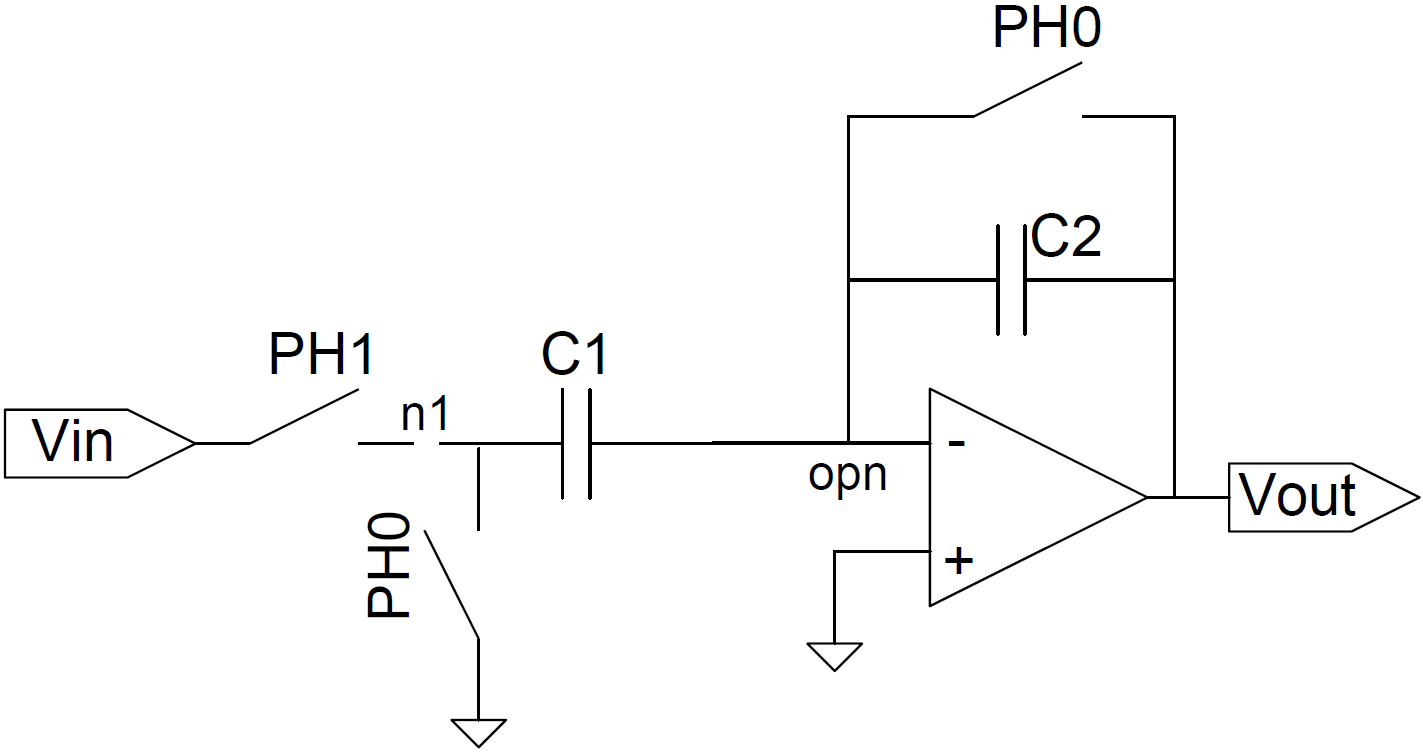
\includegraphics[width=\columnwidth]{images/invertierender_sc_verstaerker.png}
\end{minipage}
\hfill
\begin{minipage}[c]{0.58\columnwidth}
    \textbf{Hinweis:} Absolut-Werte von $C_x$ variieren um bis zu $10 \, \% $, aber \textbf{Verhältnisse} können sehr exakt sein! 
    \cbl{Verstärkung $A$}

    \begin{tabular}{@{}l l l@{}} 
        PH1   & $V_{\rm out} = 0$                   & $Q \cdot C_1 = Q \cdot C_2 = 0$ \\
        PH2   & $\Delta Q_1 = C_1 \cdot V_{\rm in}$ & $\Delta V_{\rm out} = \frac{\Delta Q_1}{C_2} = \cbl{- \frac{C_1}{C_2}} V_{\rm in}$ \\
    \end{tabular}
\end{minipage}


\subsubsection{Nicht-invertierender Verstärker}

\begin{minipage}[c]{0.4\columnwidth}
    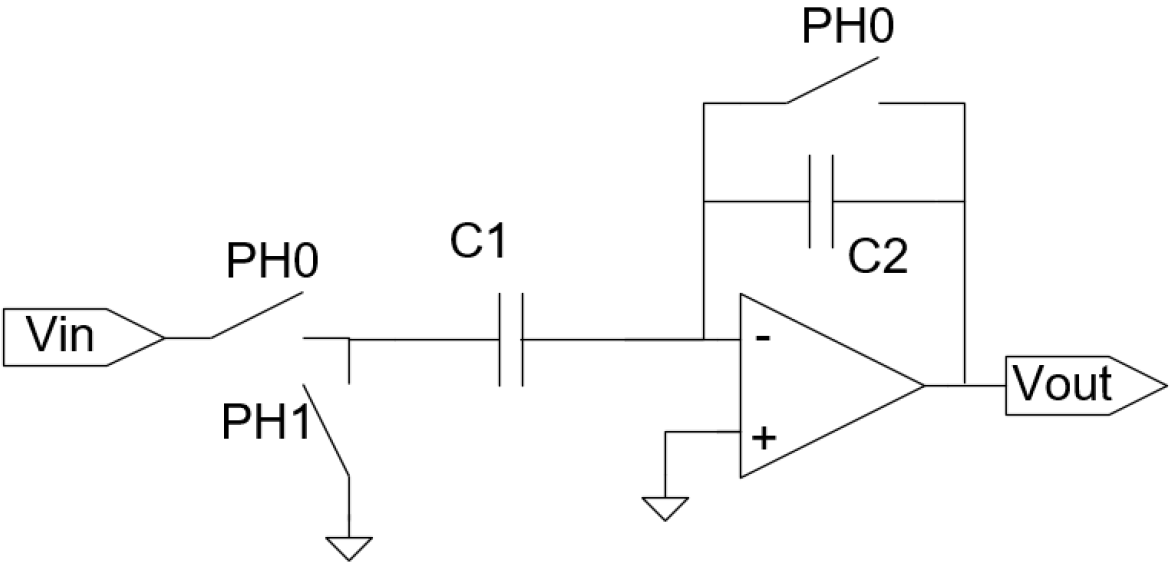
\includegraphics[width=\columnwidth]{images/nicht-invertierender_sc_verstaerker.png}
\end{minipage}
\hfill
\begin{minipage}[c]{0.58\columnwidth}
    \textbf{Hinweis:} Ansteuerung vertauscht: Aufladung von $C_1$ in PH0, gleichzeitig mit $C_2$-Reset. Ansonsten sehen der 
    invertierende und nicht-invertierende SC-Verstärker gleich aus!
    \cbl{Verstärkung $A$}
\end{minipage}

\begin{tabular}{@{}l l l l@{}} 
    PH1   & $V_{\rm out} = 0$                    & $Q \cdot C_1 = V_{\rm in} \cdot C_1$  & $ Q \cdot C_2 = 0$ \\
    PH2   & $\Delta Q_1 = -C_1 \cdot V_{\rm in}$ & $\Delta V_{\rm out} = \frac{\Delta Q_1}{C_2} = \cbl{ \frac{C_1}{C_2} } V_{\rm in}$ \\
\end{tabular}


\subsubsection{(Invertierender) SC-Integrator}

\begin{minipage}[c]{0.4\columnwidth}
    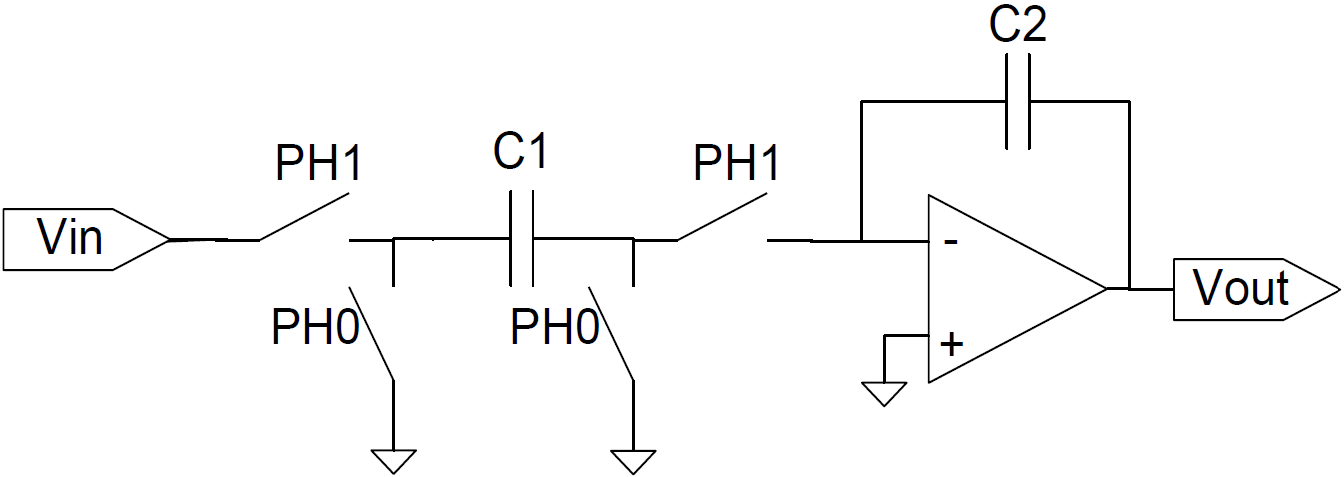
\includegraphics[width=\columnwidth]{images/sc_integrator.png}
\end{minipage}
\hfill
\begin{minipage}[c]{0.58\columnwidth}
    \begin{tabular}{@{}ll@{}}
        Spannungsänderung   & $\Delta V_{\rm out(T_n)} = - \frac{C_1}{C_2} V_{\rm in}$ \\
        Ausgangsspannung    & $V_{\rm out}(t) \cong - \frac{C_1}{C_2} \frac{1}{T} \int V_{\rm in}(t) \diff t$ \\
    \end{tabular}

    \textbf{Hinweis:} $V_{\rm out}(t)$ gilt für $t \gg T$ und langsam änderndes $V_{\rm in}$
\end{minipage}

\begin{minipage}[c]{0.25\columnwidth}
    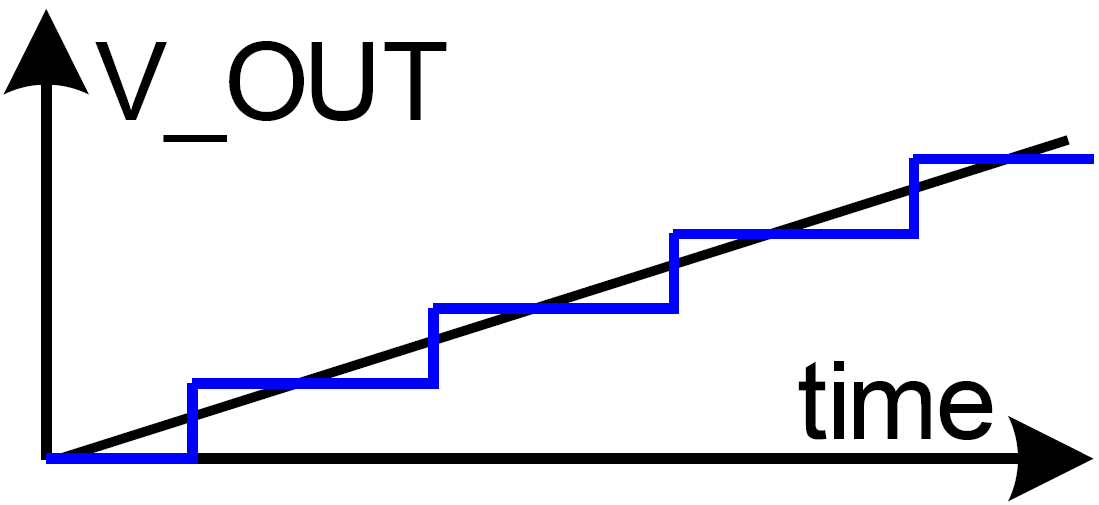
\includegraphics[width=\columnwidth]{images/sc_integrator_verlauf.png}
\end{minipage}
\hfill
\begin{minipage}[c]{0.72\columnwidth}
    \begin{itemize}
        \item In jedem Zyklus wird $C_1$ aufgeladen mit $Q = V_{\rm in} \cdot C_1$
        \item Ladungen werden in $C_2$ akkumuliert
        \item Ausgangsspannung macht Sprünge!
    \end{itemize}
\end{minipage}


\subsubsection{Nicht-invertierender SC-Integrator}

\begin{minipage}[c]{0.4\columnwidth}
    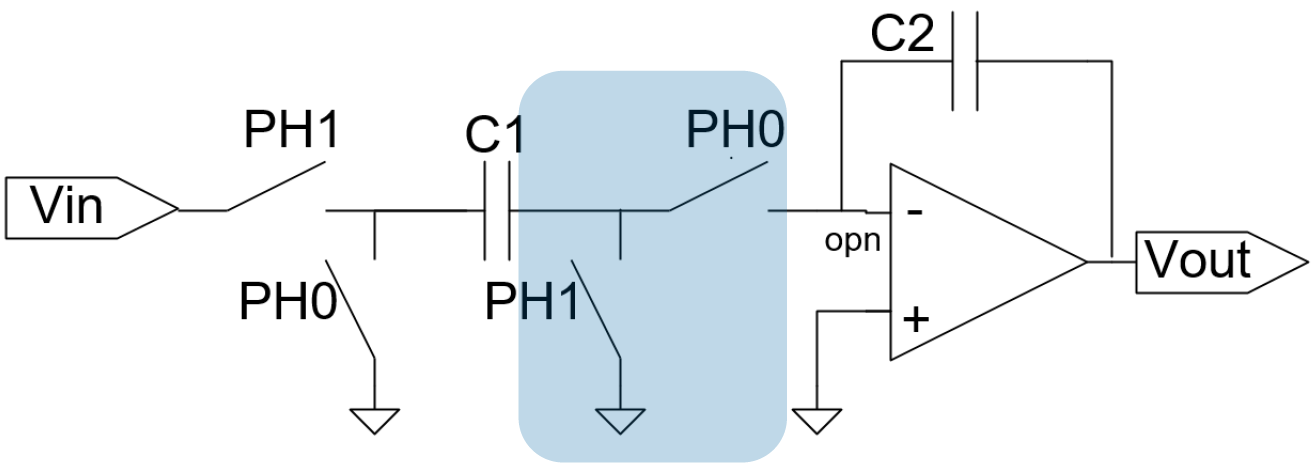
\includegraphics[width=\columnwidth]{images/nicht-invertierender_sc_integrator.png}
\end{minipage}
\hfill
\begin{minipage}[c]{0.58\columnwidth}
    \begin{itemize}
        \item Geänderte Schalter-Ansteuerung \\
            \textrightarrow\ In PH1 wird $C_1$ aufgeladen mit $V_{\rm in} \cdot C_1$
        \item In PH0 fliesst Entladestrom in $C_2$ \textrightarrow\ SC bildet einen \textbf{'negativen Widerstand'} 
            mit $R_{\rm eq} = - \frac{T_{\rm per}}{C_1}$ 
        \item \textbf{Spannungs-Sprünge sind um eine halbe Periode verschoben} 
    \end{itemize}
\end{minipage}


\subsection{Vergleich RC- und SC-Integrator}

\begin{minipage}[t]{0.55\columnwidth}
    \begin{center}
        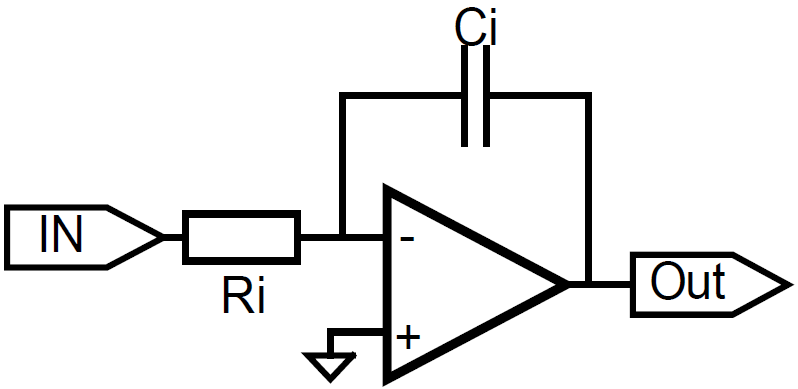
\includegraphics[width=0.55\columnwidth]{images/rc_integrator.png}
    \end{center}
    $$ V_{\rm out}(t) = - \frac{1}{R_i \cdot C_i} \int V_{\rm in}(t) \, \diff t = - \frac{1}{R_i \cdot C_i} V_{\rm in} \cdot t $$
    $$ \text{UTF:} \quad G(s) = - \frac{1}{s \cdot R_i \cdot C_i} $$
\end{minipage}
\hfill
\begin{minipage}[t]{0.42\columnwidth}
    \begin{center}
        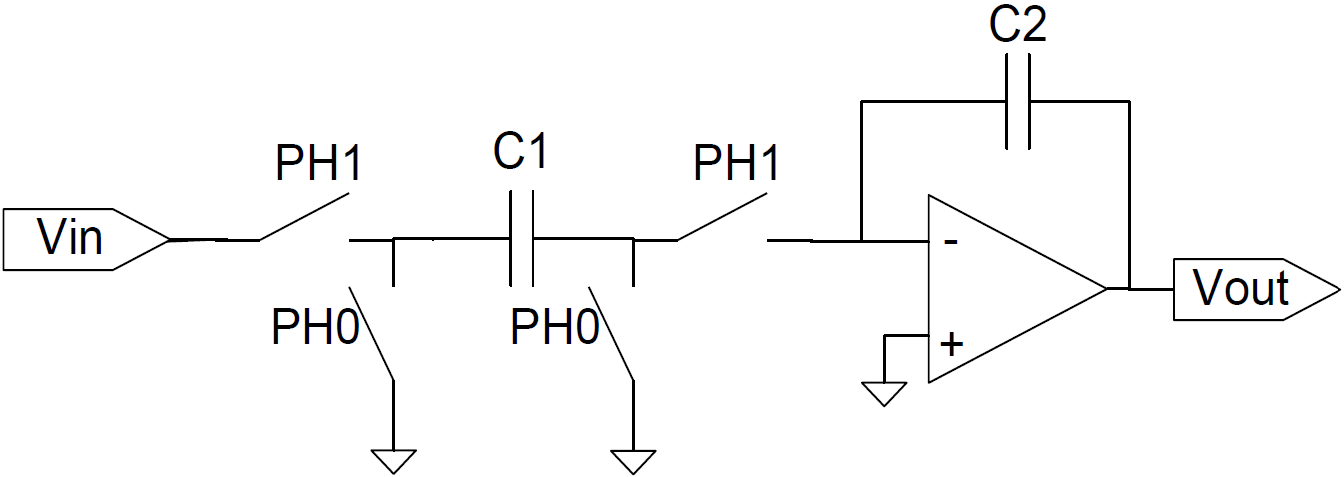
\includegraphics[width=\columnwidth]{images/sc_integrator.png}
    \end{center}
    $$ V_{\rm out}(t) = - \frac{C_1}{C_2 \cdot T} V_{\rm in} \cdot t $$
    $$ \text{UTF:} \quad G(s) = - \frac{C_1}{s \cdot C_2 \cdot T} $$
    \begin{center}
        \textrightarrow\ $R_{\rm eq} = \frac{T}{C_1}$
    \end{center}
\end{minipage}


\subsection{RC- / SC-Filter}

\begin{minipage}[t]{0.48\columnwidth}
    \begin{center}
        \myul{\textbf{RC-Filter}} 
        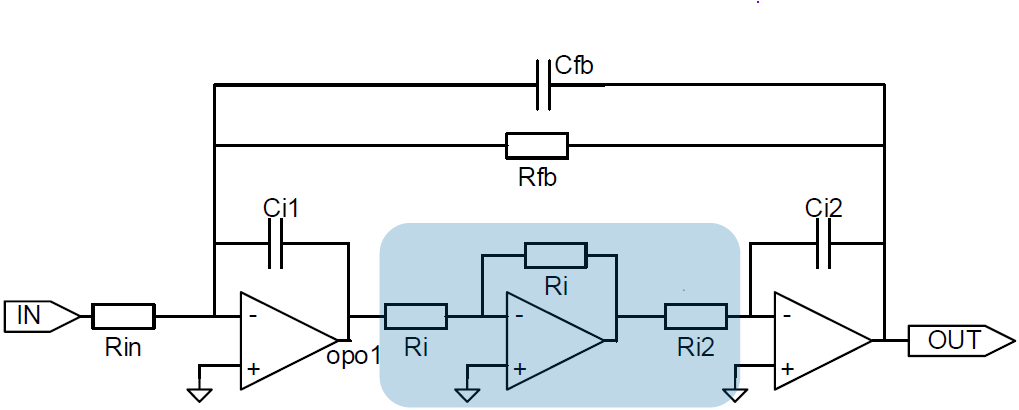
\includegraphics[width=\columnwidth]{images/rc_filter.png}
    \end{center}
    $$ \omega_0 = \frac{1}{\sqrt{C_{i1} C_{i2} R_{i2} R_{\rm fb}}} $$
\end{minipage}
\hfill
\begin{minipage}[t]{0.48\columnwidth}
    \begin{center}
        \myul{\textbf{SC-Filter}} 
        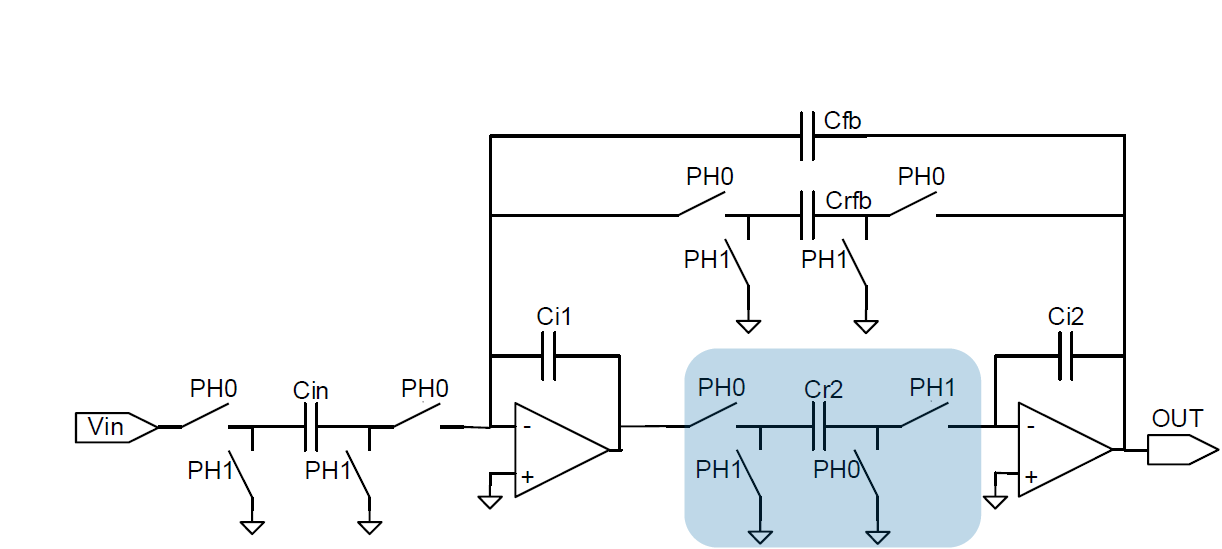
\includegraphics[width=\columnwidth]{images/sc_filter.png}
    \end{center}

    $$ \omega_0 =  \frac{1}{T} \sqrt{ \frac{C_{\rm rfb} C_{r2}}{ C_{i1} C_{i2}} } $$
\end{minipage}

\begin{outline}
    \1 Für \textbf{SC-Filter} gilt:
        \2 $C_{r2}$ wird umgekehrt angesteuert \textrightarrow\ bildet 'negativen Widerstand
        \2 Kapazitäts-Verhältnisse und Taktperiode $T$ bestimmen $f_0$ bzw. $\omega_0$
\end{outline}

\subsection{Fazit Filter}

\begin{itemize}
    \item Aktive Filter sind nötig für Polgüten $> 0.5$ (oder Spulen)
    \item Filter werden aufgeteilt in Stufen 1. oder 2. Ordnung
    \item Strukturen mit mehreren OpAmps sind weniger sensitiv auf Bauteiltoleranzen und auf Nichtidealitäten der OpAmps
    \item Als \textbf{integrierte Schaltungen} werden oft Switched-Capacitor-Schaltungen eingesetzt
\end{itemize}